\subsection{Problemas}

\subsubsection{Acesso à informações}

Foi identificado um problema de acesso à certas atividades em um fluxo de trabalho com muitas repetições por parte de médicos em sistemas LIMS. Com isso, foi elaborado uma maneira de trocar a ordem dos BPMs para maior facilidade de acesso direto à atividade desejada sem a perda de informações.

Para isso, precisamos trocar a ordem do BPM sem perder os dados da atividade, já que a própria transição entre atividades pode significar algum tipo de informação por si só (exemplo: um experimento só deve ser realizado após um outro experimento)

BPMs podem ter múltiplas atividades iniciais e múltiplas atividades finais \cite{Dijkman2008}. Utilizando desse conceito, o workflow a ser alterado foi dividido em duas partes (figura \ref{fig:realWorkflow}): 

\begin{itemize}
    \item Um evento inicial que aponta para a atividade desejada pelo usuário
    \item Um evento inicial que aponta para a atividade inicial do workflow, preenchido até a atividade escolhida para ser a nova primeira atividade inicial
\end{itemize}

\begin{figure}
    \centering
    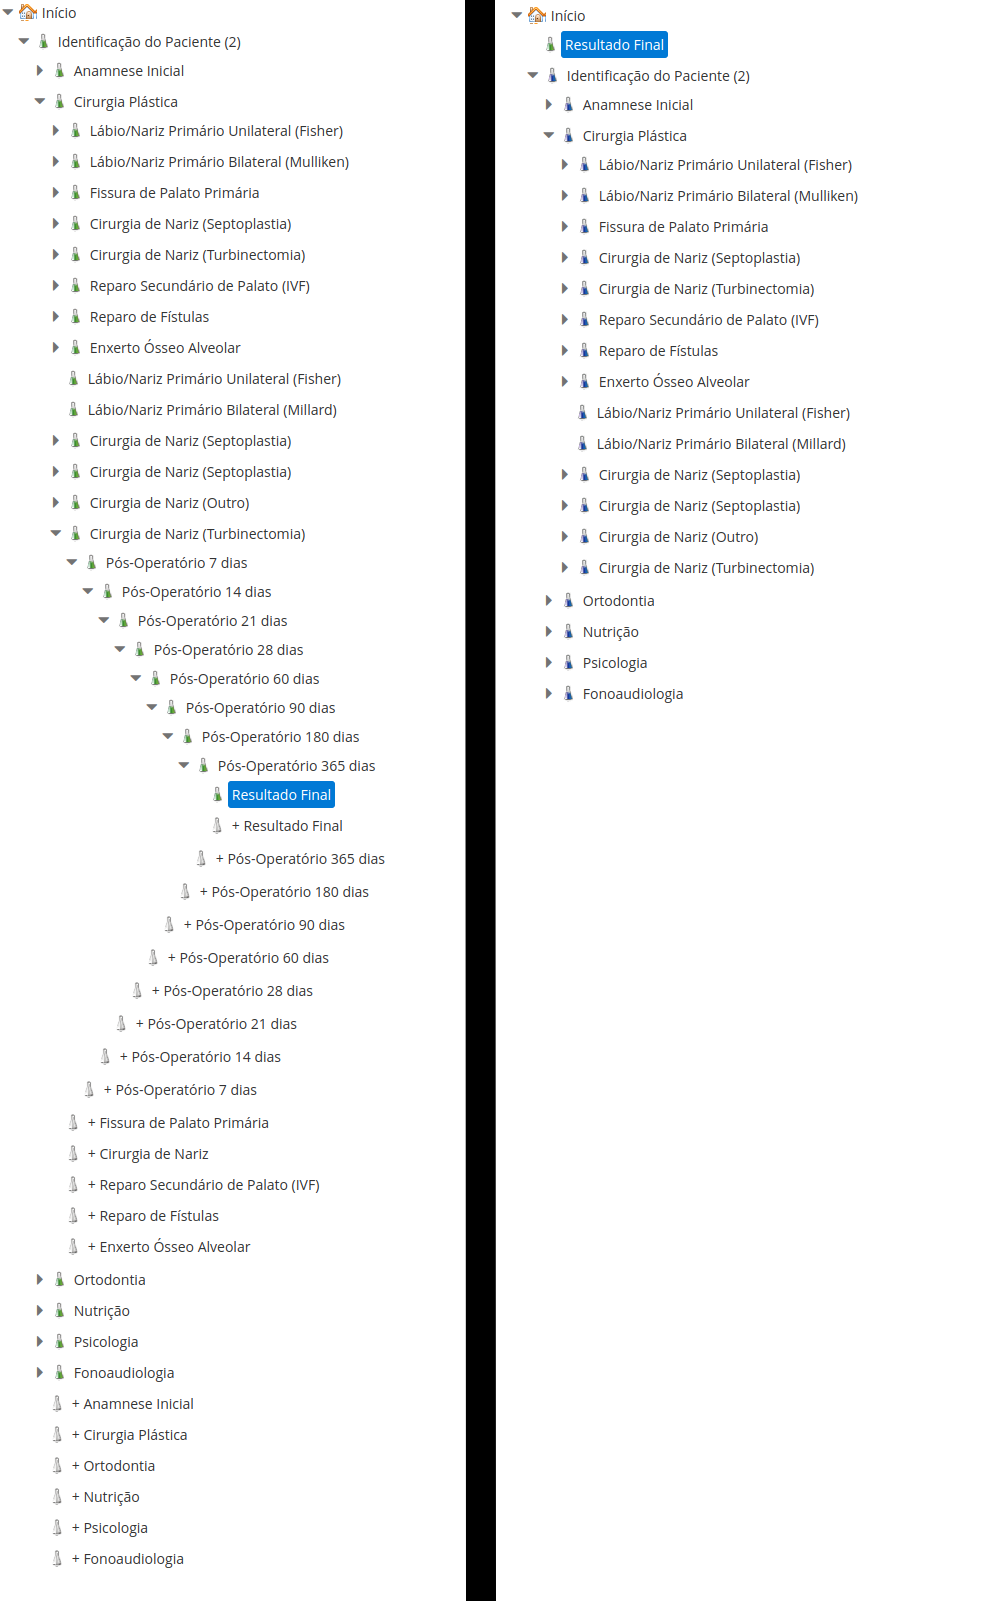
\includegraphics[width=10cm,height=15cm]{imgs/CENTRARE/arvoreNormalEAlterada.png}
    \caption{Workflow com árvore de atividades original à esquerda e workflow com árvore de atividades alterada à direita.}
    \label{fig:realWorkflow}
\end{figure}

Assim, ficam duas atividades iniciais: a primeira com a atividade que o usuário deseja preencher e continuar com seus trabalhos, e a segunda com o workflow original, contendo todas as informações necessárias para o preenchimento da atividade escolhida.

\subsection{Coleta dos dados Dados}

Foi utilizado o LIMS Flux, um LIMS generalizado que pode implementar fluxos de diversos laboratórios com uma interface gráfica presente dentro do próprio sistema \cite{Melo2010}. O Flux é uma ferramenta criada na linguagem Java, utilizando JavaServer Faces como framework de Front-end. O servidor utilizado para deploy é o Apache Tomcat.

Nele, utilizamos dados coletados de três workflows: O workflow BPL - Equipamentos, BPL - POP e o workflow CENTRARE. Os workflows BPL - Equipamentos e BPL - POP servem para controle de equipamentos e registro de informações sobre os procedimentos usados no laboratório, respectivamente, enquanto que o CENTRARE é um workflow para acompanhamento de pacientes com fissura de palato, desde o nascimento até os 20 anos, feito em conjunto com o hospital da baleia em Belo Horizonte.

Os workflows na ferramenta Flux seguem a notação de BPMs (BPMN - Business Process Model Notation) para representar os workflows implementados. Com isso, foi possível testar nesta ferramenta a troca de atividades iniciais e seu impacto nos trabalhos feitos pelo laboratório e fazer a prova de conceito sobre a alteração do fluxo de trabalho em BPMs.

Para o BPL (figura \ref{fig:bplEstrutura}), temos muitos usuários utilizando o mesmo workflow. Mas como o workflow é pouco profundo, com duas até no máximo cinco atividades de profundidade e com maior número de instâncias (ou seja, várias repetições da atividade inicial) ao invés de repetição de atividades dentro do workflow, temos que a centralização em algum atividade específica pode ajudar, mas não é muito necessária.

\begin{figure}
    \centering
    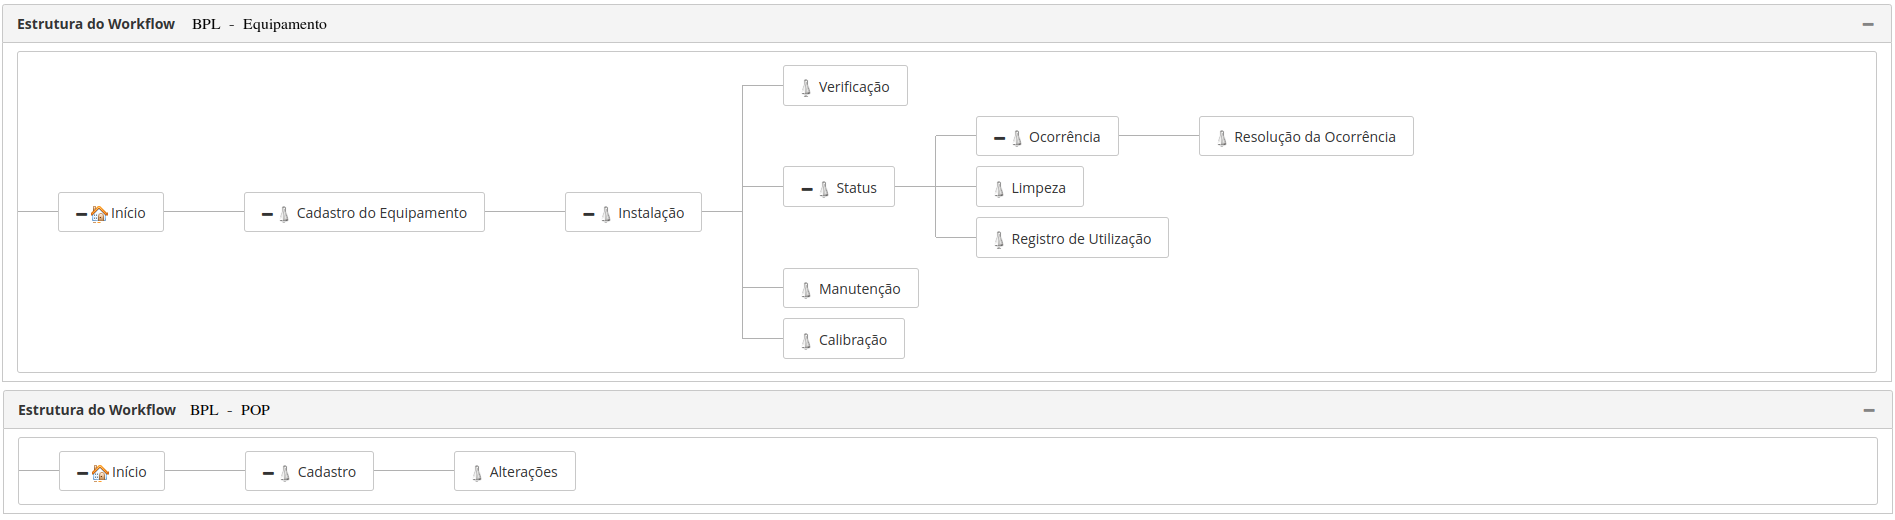
\includegraphics[width=1\textwidth]{imgs/BPL/estrutura.png}
    \caption{Estrutura dos workflows BPL - Equipamentos (Acima) e BPL - POP (Abaixo)}
    \label{fig:bplEstrutura}
\end{figure}

\subsection{Estrutura de workflows}

Para o CENTRARE (figura \ref{fig:centrareEstrutura}), temos muitos médicos que acompanham pacientes separadamente em vários setores de tratamento como cirurgia de palato, cirurgias odontológica, nutricionistas, psicólogos, fonoaudiólogos, entre muitos outros, e todas essas informações ficam em uma instância de um paciente em específico. Isso faz com que tenhamos muitas informações importantes apenas para pessoas específicas no fluxo de tratamento, com uma profundidade grande de atividades no fluxo de trabalho.

\begin{figure}
    \centering
    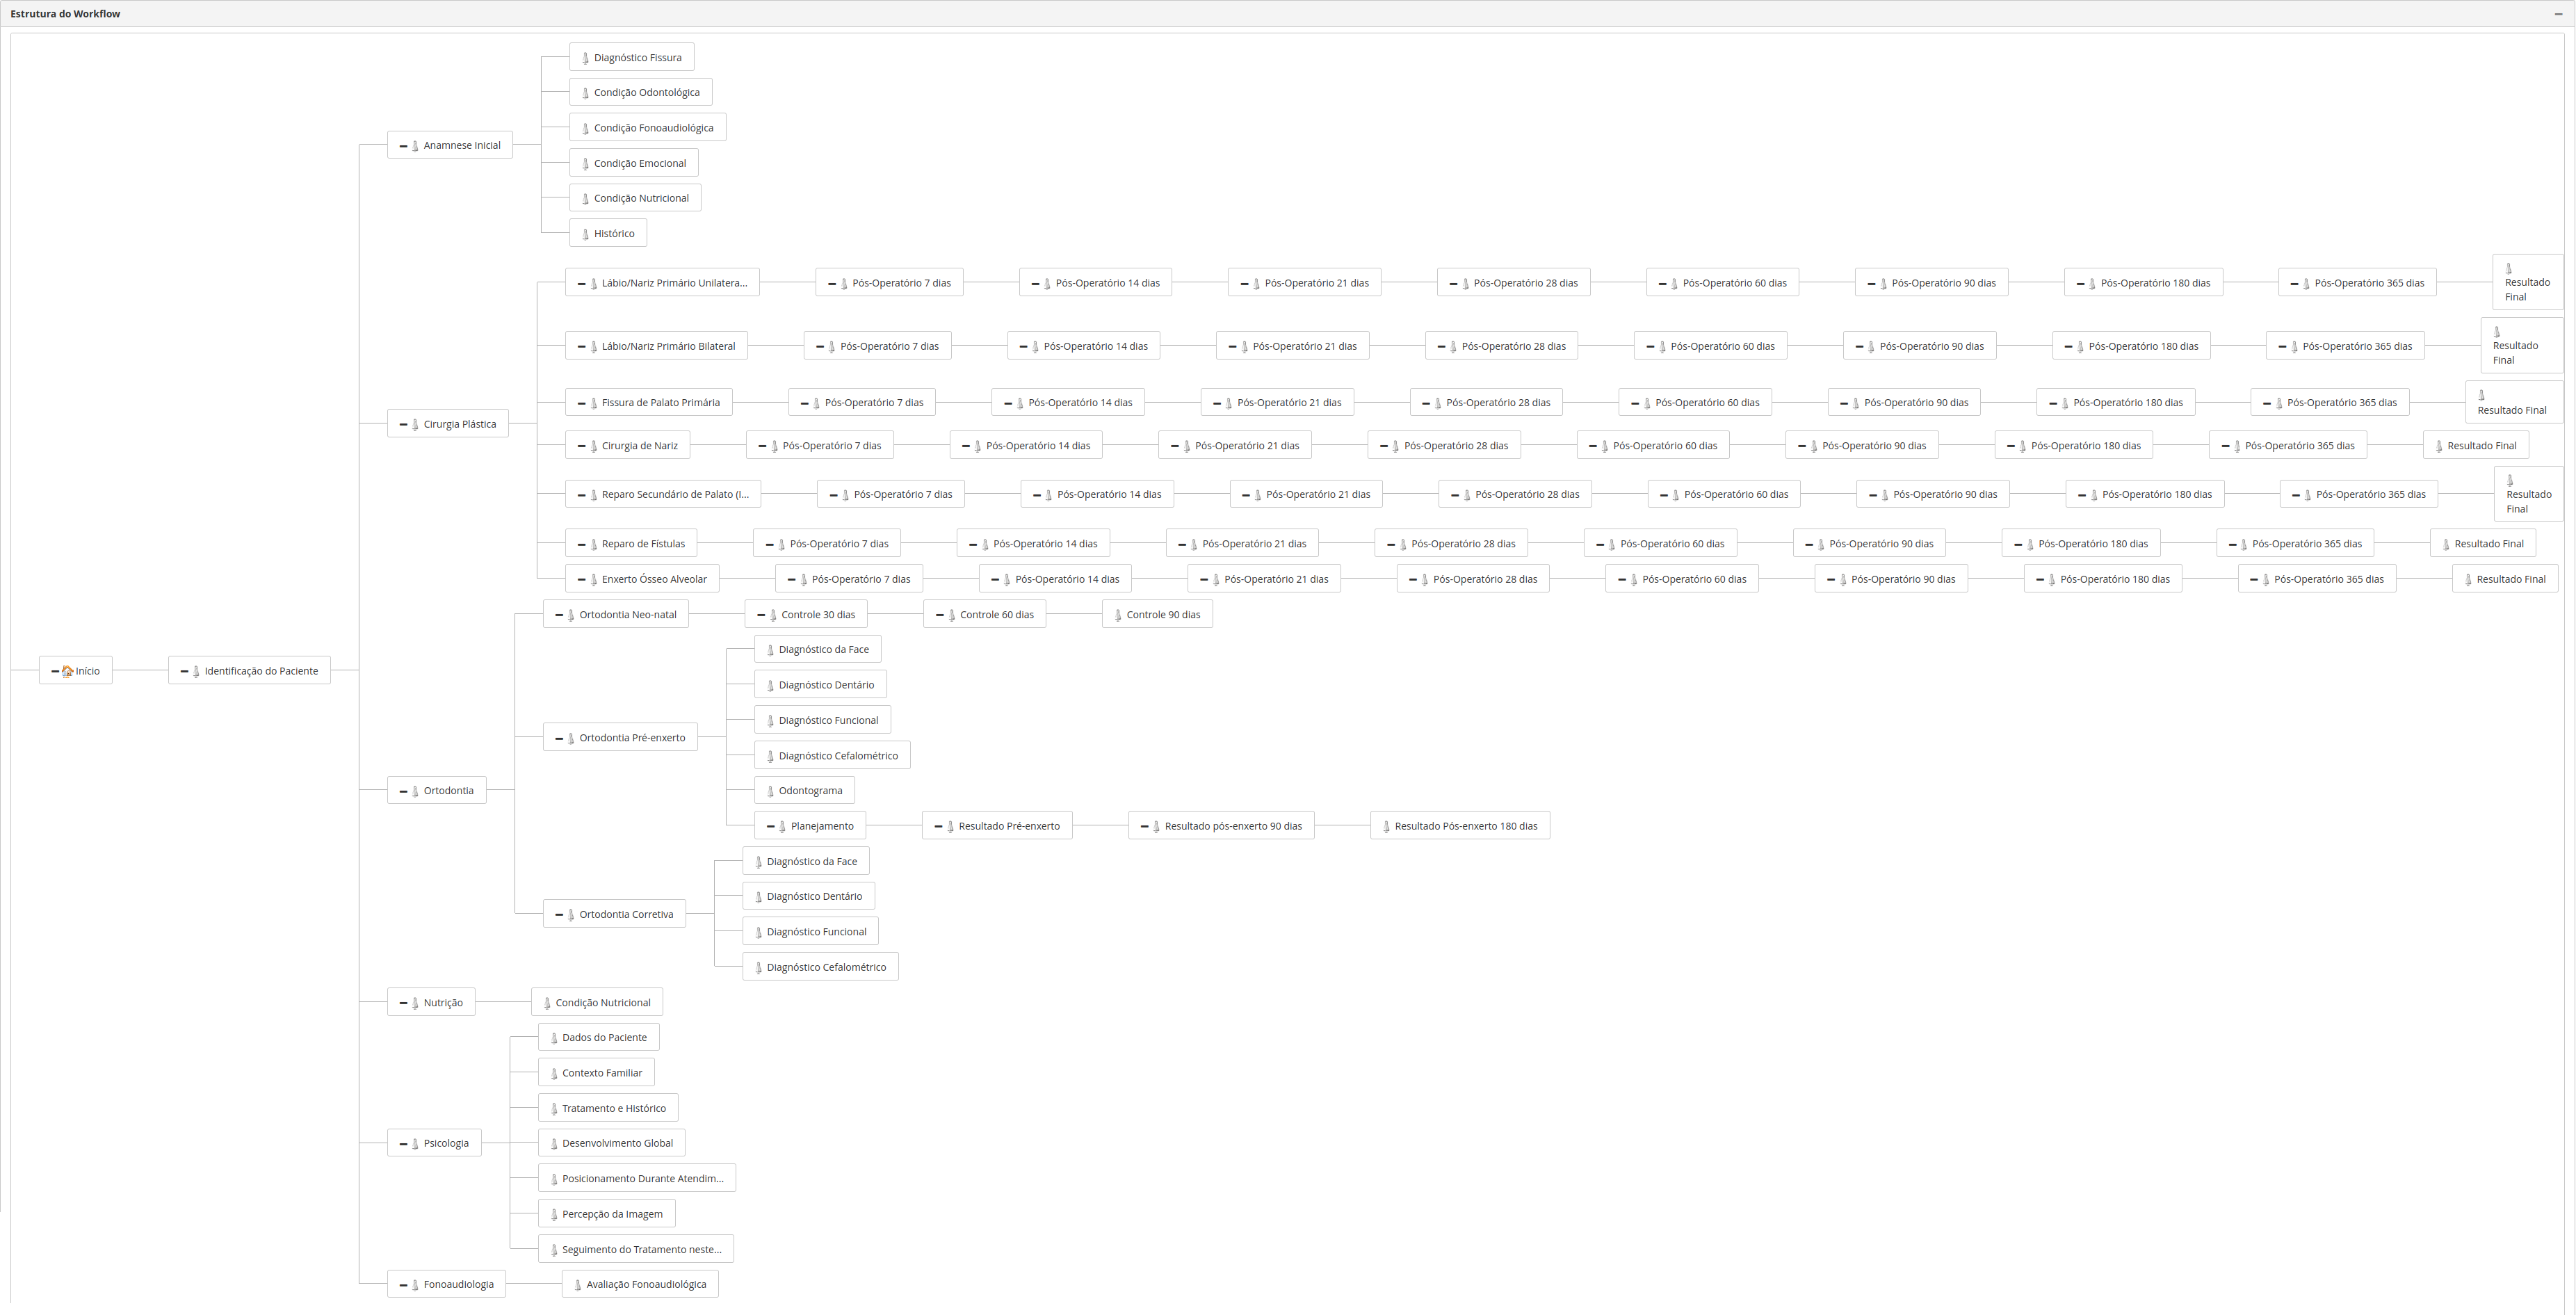
\includegraphics[width=1\textwidth]{imgs/CENTRARE/estrutura.png}
    \caption{Estrutura do workflow CENTRARE}
    \label{fig:centrareEstrutura}
\end{figure}

A centralização de atividades específicas é muito benéfica neste caso: Muitas pessoas trabalhando em partes do fluxo, mesmo que as atividades sejam dependentes de atividades anteriores, já que conseguimos "pular" atividades anteriores que podem não ser tão interessantes para a execução da atividade atual (exemplo: Um diagnóstico feito pelo ortodontista pode não ser interessante para o cardiologista) mas ainda assim obter informações necessárias com o segundo ramo de atividades criado.

Nos workflows BPL, temos dois fluxos que necessitam de compartilhamento de informações, já que um experimento não pode ser realizado se algum equipamento não for calibrado. Como não são as mesmas pessoas que trabalham no mesmo workflow (o técnico dos equipamentos não faz o experimento), com a implementação de BPMs atuais, não é possível que o cientista obtenha essa informação sem pesquisar no outro fluxo de trabalho para encontrar a informação requerida.

Com isso, o compartilhamento de atividades entre BPMs para obtenção de informações ajuda os cientistas e técnicos a automatizar a disponibilização de equipamentos quando uma calibração é realizada, um cientista pode requerir reparos de um equipamento ou o técnico pode obter dados de quantos experimentos já foram feitos em um determinado período de tempo em alguma máquina.

Como exemplo de outros workflows que são melhorados com o compartilhamento de atividades são workflows de telemedicina, onde compartilhamento de informações entre pacientes e entre profissionais de saúde é de extrema importância. Também pode ser compartilhado informações administrativas do hospital como quais leitos estão disponíveis, quais produtos (como soros ou remédios) estão disponíveis para uso e quantos médicos estão disponíveis no momento para determinada função.

Também é importante ter o compartilhamento de mensagens entre workflows de biomedicina em laboratórios, em que o compartilhamento de informações entre experimentos ajuda tanto para armazenamento de produtos quanto para os resultados que são importantes para administradores, técnicos de equipamentos e também para outros cientista que estão realizando outros experimentos. Com o compartilhamento de atividades, o administrador do laboratório pode ver quantos experimentos foram realizados em determinada data, informar técnicos que determinado equipamento necessita de manutenção e fazer controle de estoque de itens necessários para o funcionamento correto do local.

\section{Implementação}

\subsection{Centralização de atividades}

O intuito da centralização de atividades é permitir que o usuário transforme o BPM para que todas as atividades tenham a possibilidade de serem uma atividade inicial. Isso dá uma maior flexibilidade para que o acesso à informação seja feita de maneira rápida, sem ter que ser mostrado informações desnecessárias para o utilizador.

A centralização de atividades foi realizada pensando na disponibilização tanto de atividades anteriores quanto de atividades futuras para o usuário, centralizando na atividade esperada. Sem a disponibilização de atividades passadas, o usuário poderia perder informações importantes que podem (ou não) ser necessárias para o preenchimento da atividade atual.

No caso do workflow CENTRARE, a identificação do paciente fica na primeira atividade do workflow quando na orientação "original", sendo esta atividade essencial para a identificação do paciente. Além disso, a anamnese do paciente é feita em atividades filhas da identificação do paciente, tendo nela toda a informação necessária para o tratamento de tal paciente, além de conter o histórico de todas as operações e do estado atual do mesmo.

O workflow CENTRARE se beneficia imensamente desta implementação por ser um workflow muito grande e que é trabalhado por vários médicos diferentes. Assim, existem muitas informações que, para aquele médico, não são necessárias no momento (como no caso de informações do fonoaudiólogo disponíveis para o psicologo).

\subsection{Compartilhamento de atividades}

O compartilhamento de atividades foi feito para workflows com múltiplas instâncias diferentes. Para isso, recriamos os workflows BPL de uma maneira diferente: Os BPLs se tornaram um único workflow com múltiplas atividades iniciais, sendo elas uma junção do workflow BPL - Equipamento e BPL - POP: Temos o cadastro de equipamentos e de procedimentos em um mesmo workflow, sendo eles feitos por pessoas diferentes e controlados por um sistema de permissões já existente \textbf{(referência)}.

Assim, é possível compartilhar quando uma calibração de equipamento é realizada para as instâncias de procedimentos (ou para outras instâncias de calibração). O compartilhamento é feito selecionando em uma lista de instâncias disponíveis para quais instâncias o usuário gostaria que a atividade fosse mostrada. Essa seleção é feita pelo próprio usuário que completou a atividade.

Com isso, a disponibilização da atividade se torna responsabilidade do usuário, que dita para qual técnico um procedimento deve ser disponibilizado ou o contrário, um técnico seleciona para qual(is) cientista(s) uma calibração de equipamento deve ficar disponível.

Disponibilizando a atividade com diferentes níveis de permissão para diferentes usuários - médicos só podem ver diagnósticos com pacientes enquanto que técnicos de laboratório (para um possível pedido de exame de sangue, por exemplo) só podem ver o pedido de exame, calibração de equipamentos, o procedimento para a realização do pedido e com isso disponibilizar o resultado para o médico, que tem a permissão somente de visualização do resultado do exame.

Essa feature disponibiliza o compartilhamento de informações entre usuários assincronamente, tendo um sistema parecido com o de requisição (referencia) focado para BPMs

\subsection{Comparação entre implementações}

As duas features, pensados desde o começo como complementares, resolvem problemas diferentes que tomam conta dos BPMs. No caso de compartilhamento de informações entre dois workflows, ele disponibiliza o compartilhamento assíncrono de informações entre duas partes diferentes do workflow não relacionadas (Exemplo: Médico e Técnico de equipamento).

No caso de centralização de atividades, ele possibilita que todas as atividades possam ser atividades iniciais em relação a alguma instância original já criada, pulando atividades que contém informações não necessárias para o usuário em questão.

Como podemos ver na figura \ref{fig:centrare_divided}, o workflow mesmo sendo profundo, segue uma divisão entre os profissionais de saúde que trabalham nele. O problema é que todos necessitam das informações do paciente (Primeira atividade) e também das informações inseridas nas atividades nas atividades dentro da divisão em azul. Por isso a primeira atividade é bastante útil para cada um, pois podem acessar cada areá pertinente a sua especialidade e ainda manter a informação dos outros médicos disponíveis.

\begin{figure}
    \centering
    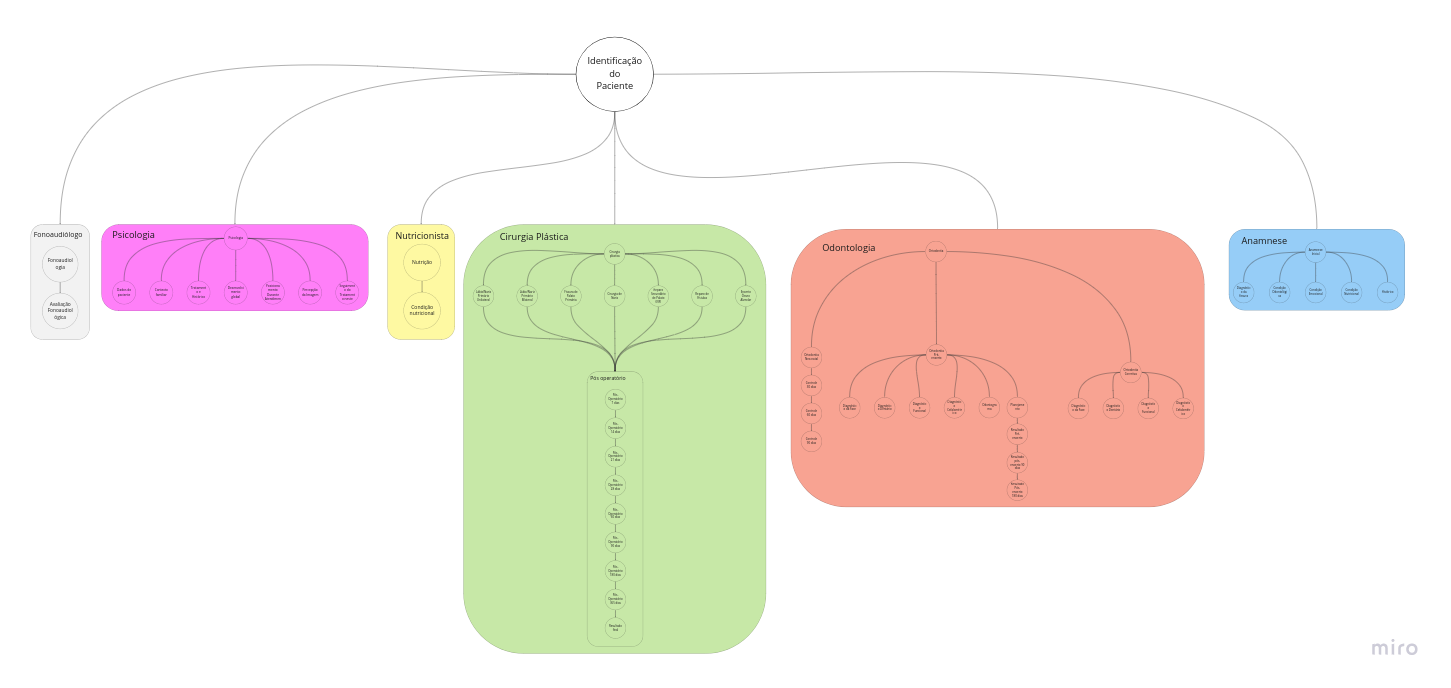
\includegraphics[width=1\textwidth]{imgs/CENTRARE/centrare.png}
    \caption{Estrutura do workflow CENTRARE dividido por atuação profissional}
    \label{fig:centrare_divided}
\end{figure}

\begin{figure}
    \centering
    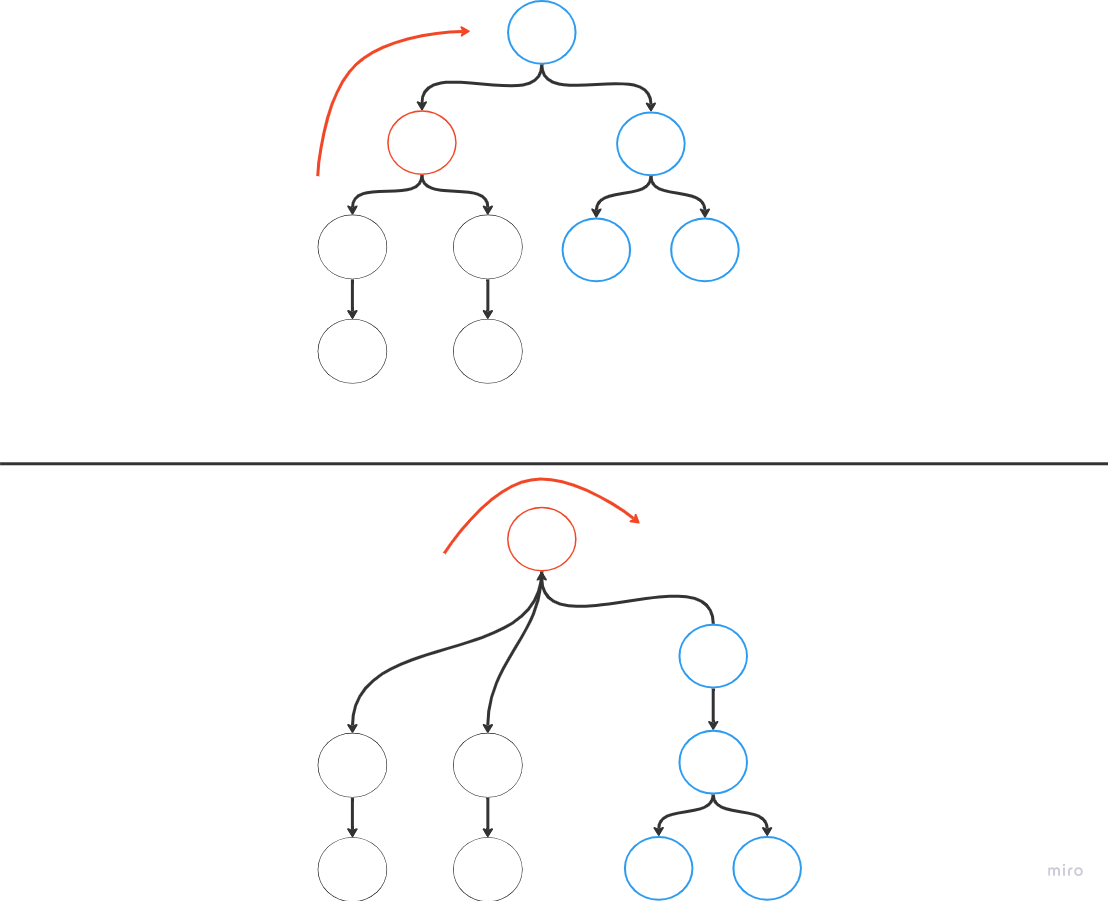
\includegraphics[width=1\textwidth]{imgs/Implementacoes/primeiraImplementacao.png}
    \caption{Representação da rotação que ocorre no workflow quando é trocada a primeira atividade. As atividades em azul são as atividades que antes faziam parte do pai da atividade selecionada (em vermelho)}
    \label{fig:primeira_implementacao}
\end{figure}

Na segunda implementação, temos na figura \ref{fig:segunda_implementacao} a representação de uma comunicação dentro de um mesmo workflow com múltiplas atividades iniciais. Esta comunicação ocorre assincronamente, já que a atividade se torna disponível para os outros usuários assim que ela é completada.

O acesso a atividades - tanto a compartilhada quanto as seguintes a ele - é controlado pelo sistema de permissões já presente no flux e seu funcionamento é explicado no artigo \textbf{Referencia}. Com isso, podemos ditar que um usuário tem acesso a atividade compartilhada e a seu resultado (círculos pretos na figura \ref{fig:segunda_implementacao}), enquanto os procedimentos realizados para se chegar no resultado estão disponíveis apenas para outro usuário (círculos vermelhos).

\begin{figure}
    \centering
    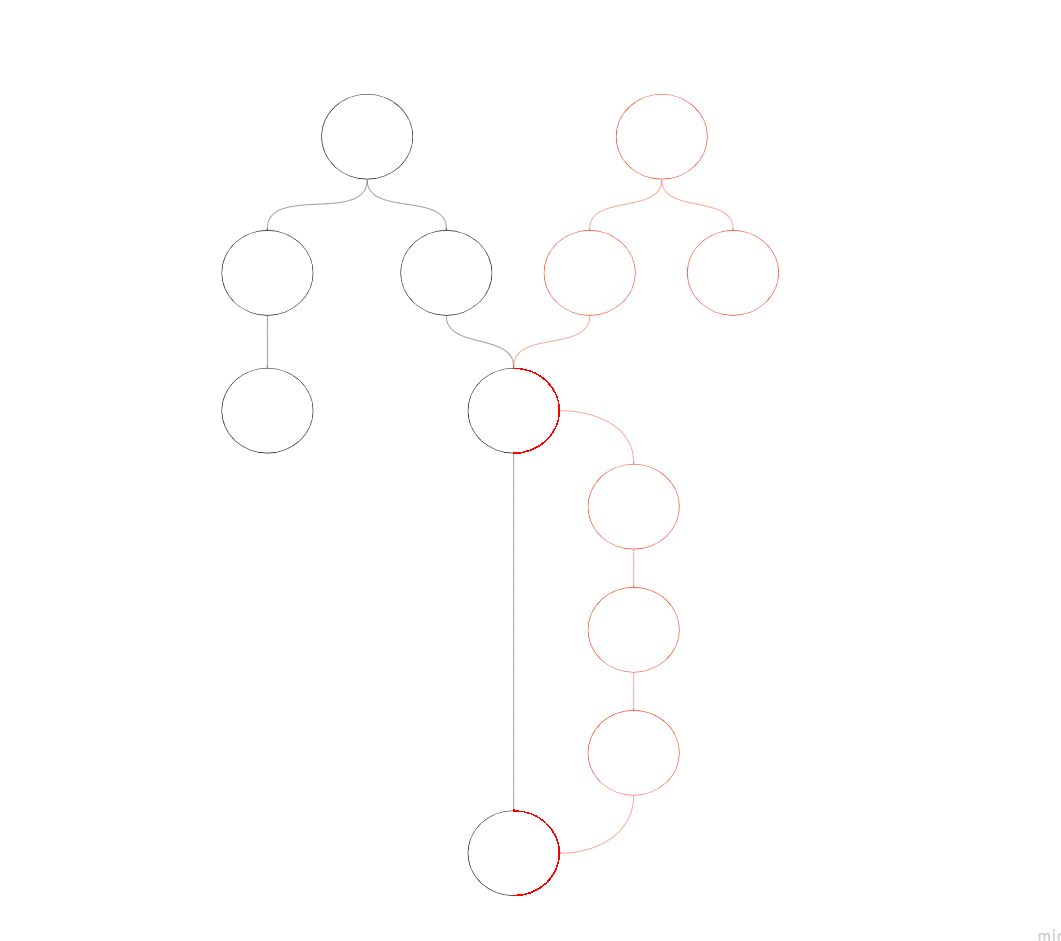
\includegraphics[width=1\textwidth]{imgs/Implementacoes/segundaImplementacao.png}
    \caption{Comunicação entre duas partes de um mesmo workflow com duas (ou mais) atividades iniciais. Atividades em preto e vermelho são atividades compartilhadas, enquanto atividades em preto estão disponíveis para um usuário A e atividades em vermelho para um usuário B.}
    \label{fig:segunda_implementacao}
\end{figure}

\subsection{Utilização das duas implementações}

Com a utilização das duas implementações, usuários diferentes podem ter seus próprios workflows e também utilizar da função de busca e alteração de atividade inicial para encontrar mais rapidamente o fluxo de trabalho que será feito no momento (mudar).

